\documentclass{article}
\usepackage{fullpage, tikz, calculator, amsmath, tocloft, floatrow, caption, subcaption, tcolorbox,colortbl,multicol}
\tikzstyle{bigdot}=[shape=circle,minimum size=3mm,inner sep=0,very thick,draw,fill=yellow]
\tikzstyle{smalldot}=[gray,shape=circle,minimum size=1mm,inner sep=0,fill,draw]
\usepgflibrary{patterns}


%in case I want to give them better names later
\newcommand{\rk}{rectangle example knot}
\newcommand{\RK}{Rectangle Example Knot}
\newcommand{\sk}{square example knot}
\newcommand{\bk}{border example knot}
\newcommand{\SK}{Square Example Knot}
\newcommand{\BK}{Border Example Knot}

\newcommand{\gen}{\hyperref[generated]{$^*$}}%link to citation for pictures generated by website

%
\usetikzlibrary{shapes.geometric, arrows}
\usetikzlibrary{decorations.pathreplacing}
\tikzstyle{startstop} = [rectangle, rounded corners, minimum width=3cm, minimum height=1cm,text centered, draw=black, fill=red!30]
\tikzstyle{io} = [rectangle, minimum width=1cm, minimum height=1cm, text centered, draw=black, fill=blue!30]
\tikzstyle{process} = [rectangle, minimum width=3cm, minimum height=1cm, text centered, draw=black, fill=orange!30]
\tikzstyle{decision} = [trapezium, trapezium left angle=70, trapezium right angle=110, text centered, draw=black, fill=green!30]
\tikzstyle{arrow} = [thick,->,>=stealth]


\usepackage{listings}%for pasting in python code
\usepackage[colorlinks,linktoc=page,linkcolor=blue]{hyperref}
%\renewcommand{\cftsubsecaftersnumb}{\hspace{1.5em}}

\newcommand{\summ}[1]{%add summaries to table of contents
%subsection standard indent is 1.5 em; adding an initial space avoids hanging indents
%\phantomsection
\addcontentsline{toc}{subsection}{~\hspace{1.5em} #1}
}

\newcommand{\intersection}[3]{
\draw (#1,#2) node[fill=white,fill opacity=0.5,shape=circle,draw,inner sep=1mm]{#3};
\draw[] (#1,#2) node{#3};
}
\newcommand{\smintersection}[3]{
\draw (#1,#2) node[fill=white,fill opacity=0.5,shape=circle,draw,inner sep=0.5mm]{\tiny #3};
\draw[] (#1,#2) node{\tiny #3};
}

\newcommand{\ch}{}%chain
\renewcommand{\sc}{}%single crochet
\title{Crocheted Knotwork}
\author{Elyse Yeager}
\date{}

\newcommand{\m}[1]{$\stackrel{{\text{#1}}}{/}$}


\begin{document}

%%%%%%%%%%%%x


%%%%%%%%%%%%

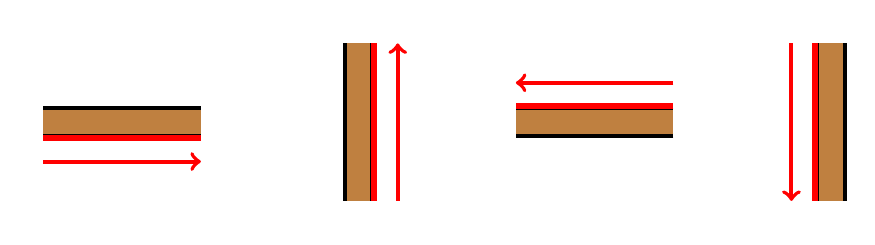
\begin{tikzpicture}
\foreach \n in {0,1,2,3}{
	\MULTIPLY{\n}{90}{\r}
	\MULTIPLY{\n}{3}{\x}
	\begin{scope}[xshift=\x cm,rotate=\r]
	\draw[line width=4mm] (-1,0)--(1,0);
	\draw[line width=3mm,brown] (-1,0)--(1,0);
	\draw[red,line width=.75mm] (-1,-.2)--(1,-.2);
	\draw[red, line width=.5mm,->] (-1,-.5)--(1,-.5);
	\end{scope}
}
\end{tikzpicture}
%%%%%%%%%%%%




%%%%%%%%%%%%

%%%%%%%%%%%%%%%%%%
%%%%%%%%%%%%%%%%%%
%%%%%%%%%%%%%%%%%%
%%%%%%%%%%%%%%%%%%

%%%%%%%%%%%%

%%%%%%%%%%%%

\end{document}


%%%%%%%%%%%%
\begin{tikzpicture}
\draw(0,0)node{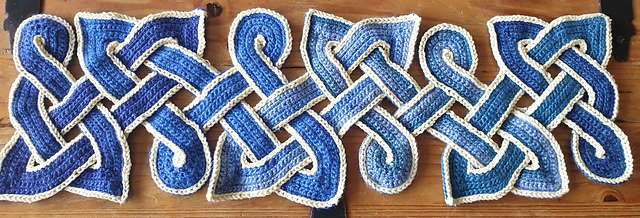
\includegraphics[width=8cm]{pic/border2}};
\foreach \n in {0,0.05,...,1}{
	\MULTIPLY{\n}{10}{\xx}
	\ADD{\xx}{-3}{\x}
	\begin{scope}
		\clip (\x,-1.5)rectangle(\x+.5,1.5);
		\MULTIPLY{\n}{2}{\o}
		\draw[opacity=\o] (-1.25,0)node{
\includegraphics[width=10cm]{border2}};
	\end{scope}
	}	
\end{tikzpicture}
%%%%%%%%%%%%



%%%%%%%%%%%%
\begin{tikzpicture}
\draw(0,0)node{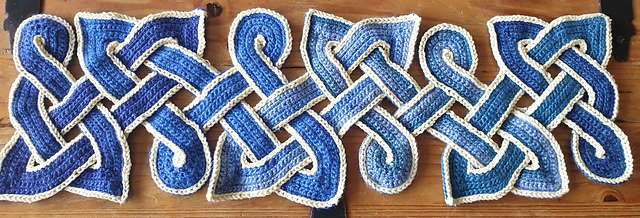
\includegraphics[width=8cm]{pic/border2}};
\foreach \n in {0,0.05,...,1}{
	\MULTIPLY{\n}{10}{\xx}
	\ADD{\xx}{-3}{\x}
	\begin{scope}
		\clip (-\x,-1.5)rectangle(-\x-.5,1.5);
		\MULTIPLY{\n}{2}{\o}
		\draw[opacity=\o] (1.25,0)node{
\includegraphics[width=10.5cm]{border2}};
	\end{scope}
	}	
\end{tikzpicture}
%%%%%%%%%%%%